\subsection{Ruby on Rails}
\label{tag:rails}
本研究で提案したネットワークシミュレータは、Ruby on Railsを用いて実装されている。Ruby on Railsとは、Rubyで構築された、Webアプリケーションを開発するためのフレームワークである。特徴としてMVCアーキテクチャの採用や設定より規約という設計哲学などが挙げられる。\\
 MVCとは「Model」,「View」,「Controller」の頭文字であり、MVCアーキテクチャとはアプリケーションの構成が以下の図\ref{fig:MVC}のように分類することに由来している。


\begin{figure}[htbp]
  \begin{center}
    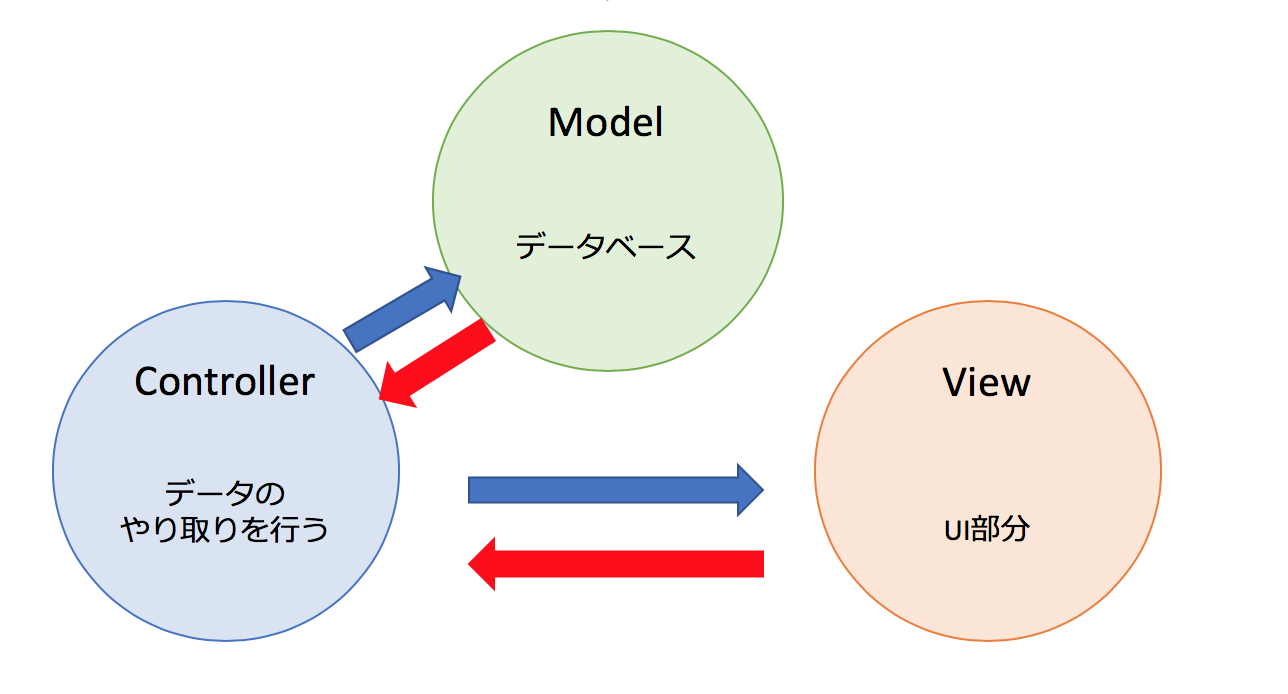
\includegraphics[clip,width=12.0cm,height=8.0cm]{img/mvc.png}
    \caption{MVCアーキテクチャ}
    \label{fig:MVC}
  \end{center}
\end{figure}

ここで「Model」とはデータベースに収めたデータやそのデータのルールなどを表す。「View」は、アプリケーションのUIの部分を指す。HTMLやCSSを用いて配置やデザインを決定する。「Controller」はViewとModelの間を取り持つ部分である。ModelとViewの間でデータの受け渡しなどを行う。\\
 Ruby on Railsではこれら「Model」,「View」,「Controller」が機能として独立しているため、それぞれの部分の開発を効率良く行うことができ、仕様変更や新たな機能の追加が容易に行える。また、「View」としてUI部分が独立しているためUIの変更も容易である。
